\section{Discussion}
\AP\label{sec:discussion}

Several open problems are left by our work, more prominently, the complexity gap for "CRPQ minimization". Below we discuss further avenues for future research.

\subsection{Variable minimization}
\AP\label{sec:varmin}

Another approach for an algorithm for query answering of a "(U)CRPQs" $\gamma$ on a "graph database" $G$ is by first guessing a variable assignment $f: \vars{\gamma} \to \vertex{G}$ and then checking, for each "atom" $x \atom{L} y$ of $\gamma$, that there is a path in $G$ from $f(x)$ to $f(y)$ with label in $L$. 

This implementation approach privileges minimizing the number of \emph{variables} as opposed to the number of \emph{atoms} of a "(U)CRPQ", and gives rise to the corresponding \reintro{variable-minimization problem(s)}. From a practical perspective, as already mentioned in the Introduction, systems commonly evaluate CRPQs via join algorithms. Recent \emph{worst-case optimal} joins algorithms work by ordering the variables and assigning potential values to these, and hence the number of variables may also be a relevant parameter in these cases~\cite{CucumidesReutterVrgoc2024SizeBounds,VrgocEtal2024MillenniumDB}. 
 % 
\decisionproblem{""Variable-minimization problem"" for "CRPQs" ("resp" for "UCRPQ")}
{A finite alphabet $\A$, a  "CRPQ" ("resp" "UCRPQ") $\gamma$ over $\A$ and $k \in \N$.}
{Does there exists a "CRPQ" ("resp" "UCRPQ") $\delta$ over $\A$ with at most $k$ variables 
("resp" whose every "CRPQ" has at most $k$ variables) "st" $\gamma \semequiv \delta$?}
As before, a "(U)CRPQ" is \AP""variable minimal"" if there is no "equivalent" "(U)CRPQ" smaller in the number of variables.

It is worth observing that for "conjunctive queries" (and for "tree patterns") minimizing the number of variables or minimizing the number of atoms is equivalent: a query is minimal in the number of variables "iff" it is minimal in the number of atoms.
However, for "CRPQs" and "UCRPQs" it is not: $\gamma(x,y) = x \atom{a} y \land x \atom{a+b} y$ is "variable minimal", but it is not (atom) "minimal" since it is "equivalent" to $\gamma'(x,y) = x \atom{a} y$. We further conjecture that there are (atom) "minimal" "CRPQs" which are not "variable minimal".
\begin{restatable}{conjecture}{conjAtomVariableMinimal}
  There exist (atom) "minimal" "CRPQs" which are not "variable minimal".
\end{restatable}

By adaptations of the algorithms of \Cref{sec:upperCRPQ,sec:upperUCRPQ} we can derive some upper bounds, which are likely to be sub-optimal.
\begin{theorem}
  The "variable-minimization problem" for "CRPQs" is in "4ExpSpace" and for "UCRPQs" in "2ExpSpace". Both problems are "ExpSpace"-hard.
\end{theorem}

\begin{proof}
  For the case of "CRPQ" "variable-minimization problem", it suffices to observe, in the proof of \Cref{lemma:crpq-size-bound}, that since each NFA of the proof has size double-exponential, there there cannot be more than a triply-exponential number of distinct NFA, and hence that the underlying multigraph of queries to be considered has a triply-exponential number of edges. Thus, there are `only' a quadruply-exponential number of such triply-exponential queries. For each such query we test if it is equivalent to the original query in "4ExpSpace".

  For the case of "UCRPQ" "variable-minimization problem", let $\+C_k$ be the (infinite) set of multigraphs having at most $k$ vertices. Via the same argument as in the proof of \Cref{lemma:approximation-for-finclass}, 
  we obtain that each $\CRPQ[\+C_k]$ in the union of "CRPQs" expressing
  $\AppInf{\Gamma}{\+C_k}=\App{\Gamma}{\+C_k}{O(\nbatoms{\Gamma}\cdot r_{\Gamma}\nbatoms{\+C})}$
  has atoms consisting in a concatenation of
  at most $O(\nbatoms{\Gamma}\cdot\nbatoms{\+C})$ "sublanguages" of $\Gamma$. Hence, there cannot be more than $2^{O(\nbatoms{\Gamma}\cdot\nbatoms{\+C})}$ distinct atoms between two variables, and $\App{\Gamma}{\+C_k}{O(\nbatoms{\gamma}\cdot r_{\Gamma}\cdot \nbatoms{\+C})} \semequiv \App{\Gamma}{\+C'_k}{O(\nbatoms{\Gamma}\cdot r_{\Gamma}\nbatoms{\+C})}$ for $C'_k$ being the finite subclass of $\+C_k$ having graphs with no more than $2^{O(\nbatoms{\Gamma}\cdot\nbatoms{\+C})}$ parallel edges.
  Hence, there is a double-exponential number of exponential queries to test for "equivalence" with $\Gamma$, which yields a "2ExpSpace" upper bound.


  The lower bounds follow by a similar idea to \Cref{thm:minimization-lowerbound} and can be found in \Cref{apdx-sec:lowerbound-variables}.
\end{proof}


\subsection{Tree patterns}
\AP\label{sec:apdx-tree-patterns}

We believe that the techniques of \Cref{sec:upperUCRPQ} should also yield a method to compute "maximal under-approximations" for unions of tree patterns, as well as a "PiP2" upper bound for the minimization problem of unions of tree patterns, contrasting with
the "SigmaP2"-completeness of minimization of tree patterns 
proven by Czerwiński, Martens, Niewerth \& Parys \cite[Theorem 3.1]{CzerwinskiMartensNiewerthParys2018Minimization}.
\todo{``We leave the details for a future long version of this article.''}

A \AP""tree pattern""---see "eg" \cite[\S 2.2]{CzerwinskiMartensNiewerthParys2018Minimization}---over node variables
$\A$ is a directed tree, whose nodes have a label from $\A\sqcup\{*\}$, and whose
edges are partition into simple edges and transitive edges.

\begin{figure}
	\centering
	\subfloat[A "tree pattern" $\tau$. Double arrows represent transitive edges.]{
		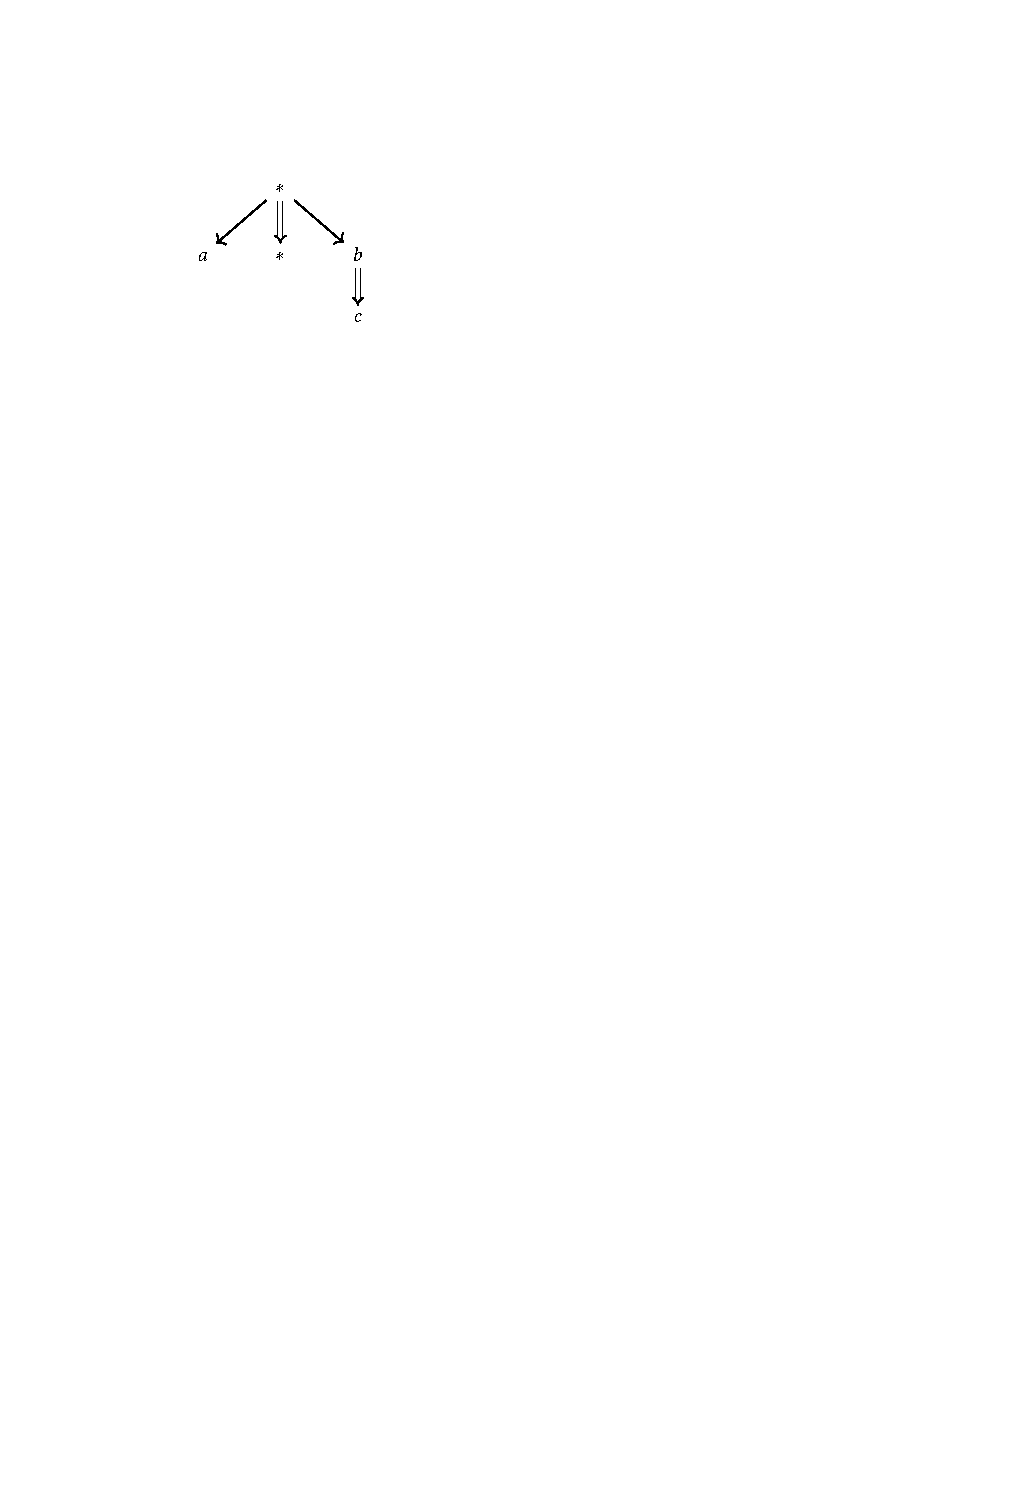
\includegraphics{fig/minimization-crpq/tree-pattern-example.pdf}
	}
	\hfil
	\subfloat[Its "encoding" $\Encoding(\tau)$ as a "CRPQ".]{
		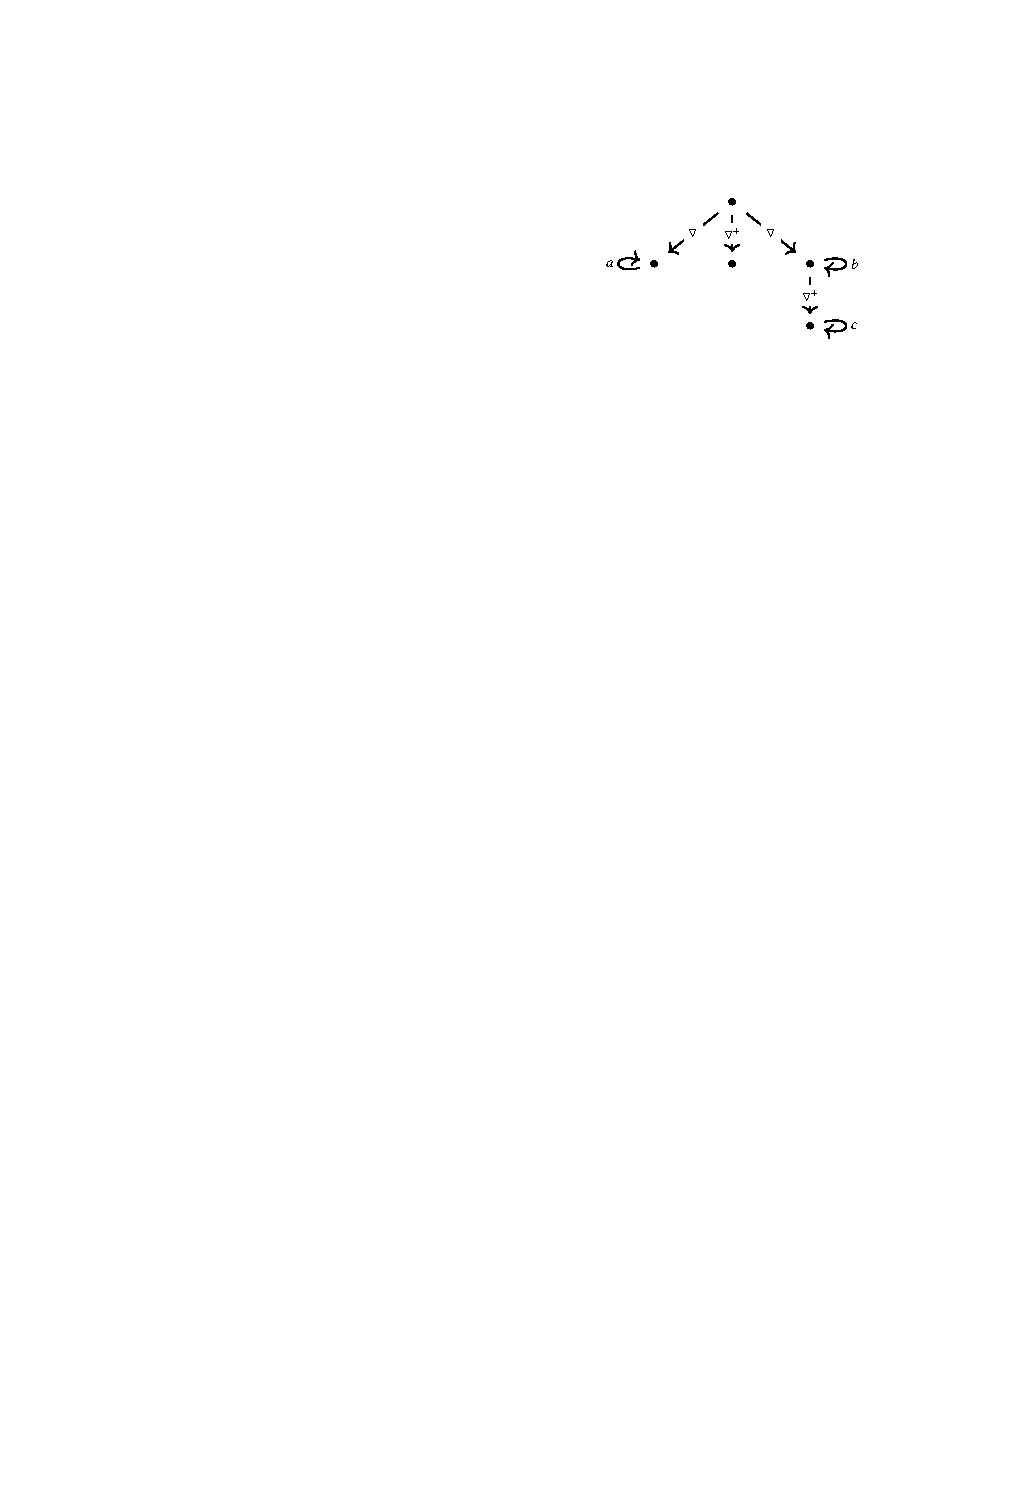
\includegraphics{fig/minimization-crpq/tree-pattern-example-enc.pdf}
	}
	\caption{
		\AP\label{fig:encoding-tree-pattern}
		"Encoding" a "tree pattern" into a "CRPQ".
	}
\end{figure}

We \AP""encode"" a "tree pattern" $\tau$ into a "CRPQ" over $\A\sqcup\{\marking\}$, denoted
by \AP$\intro*\Encoding(\tau)$, obtained as follows:
\begin{itemize}
	\item we start from the underlying tree of the "tree pattern",
		and replace simple edges by an "atom" $\qvar \atom{\marking} \qvar$,
		and transitive edges by an "atom" $\qvar \atom{\marking^+} \qvar$;
	\item for any node $x$ with a node label $a \in \A$, we add an "atom" $x \atom{a} x$;
	\item for any node with a wildcard label $*$, we do not add any "atom".
\end{itemize}
See \Cref{fig:encoding-tree-pattern} for an example. Note that this "encoding" is injective.

\begin{proposition}
	Given two "tree patterns" $\tau_1$, $\tau_2$ over $\A$, the following are equivalent:
	\begin{itemize}
		\item $\tau_1 \contained \tau_2$ as "tree patterns"---in the sense of
			\cite[Definition 2.2]{CzerwinskiMartensNiewerthParys2018Minimization}, and
		\item $\Encoding(\tau_1) \contained \Encoding(\tau_2)$ as "CRPQs".
	\end{itemize}
\end{proposition}

\begin{proof}[Proof sketch]
	This follows from the characterization of containment for "tree patterns"
	using ``canonical tree models''---see \cite[\S4.2]{CzerwinskiMartensNiewerthParys2018Minimization}\footnote{Note
	however that the authors assume the set of labels to be infinite, and label `$*$'-nodes
	by $z$-nodes where $z$ is a new label: this assumption can be removed by
	allowed unlabelled nodes in the model.}---and the characterization of "containment" for "CRPQs"
	via "canonical databases" ("aka" "expansions")---see \Cref{prop:cont-char-exp-st}.
\end{proof}

We do not fully understand the relation between tree pattern minimization and "CRPQ minimization", 
and conjecture that this encoding actually preserves minimality, but we have failed so far to prove this. 

\begin{restatable}{conjecture}{conjTreePatternsAsCRPQs}
	If a "tree pattern" is minimal among "tree patterns", 
	then its "encoding" as a "CRPQ" should also be minimal among "CRPQs", up to "contracting internal variables".
\end{restatable}